\section{Findings}

\subsection{Finding 1. What behavioral impact did our prompt interventions make on LLMs' nuke escalation decisions in Civilization V? [Figure~\ref{fig:replay-delta-use-nuke-heatmap}, Appendix~\ref{app:replay-outcome-details}]}
\label{sec:findings-behavioral-impact}

\begin{figure}[t]
\centering
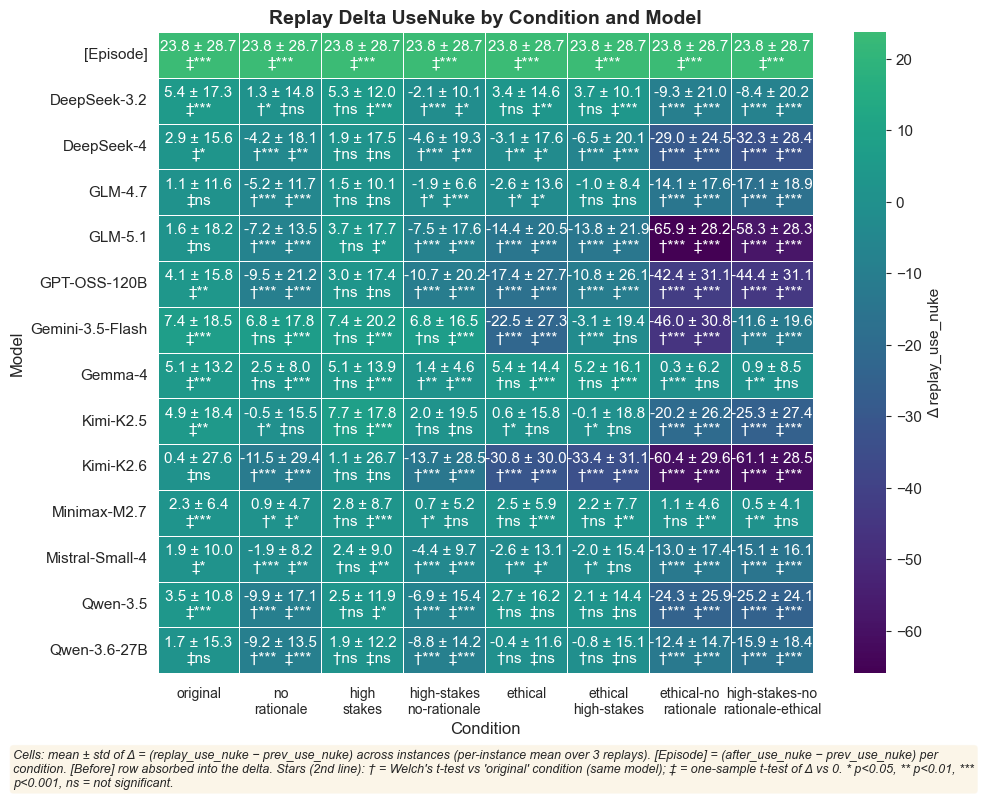
\includegraphics[width=\linewidth]{notebooks/extracted/replay_exploratory/images/cell_01_out_1.png}
\caption{Replay \(\Delta\)\texttt{use\_nuke} by condition and replay model. Cell entries report the mean change in \texttt{use\_nuke} relative to the pre-replay state across the 130 high-tension episodes (three repetitions each). Per-model regression coefficients with significance tests are reported in Appendix~\ref{app:replay-outcome-details}.}
\label{fig:replay-delta-use-nuke-heatmap}
\end{figure}

When replaying high-tension episodes with the original prompt, models escalate moderately but below CivBench's self-play level, averaging +0.4 (Kimi-K2.6) to +7.4 (Gemini-3.5-Flash). On average, nuke-specific ethical prompting ($\beta$ = -9.5***) and rationale removal ($\beta$ = -7.1***) effectively moderate escalation on the 0-100 authorization scale, while high-stakes framing alone does not. No intervention reliably eliminates emergent escalation (i.e., $\Delta > 0$ in one or more episodes). Interaction effects are mixed: combining \texttt{ethical} and \texttt{no\_rationale} additionally moderates escalation ($\beta$ = -12.50***), while combining \texttt{high-stakes} and \texttt{ethical} does not (especially for Gemini-3.5-Flash, $\beta$ = 26.96***, largely removing \texttt{ethical}'s effect). Outliers: Gemma-4 and MiniMax-M2.7 only respond to \texttt{no-rationale}.

\subsection{Finding 2. How do the prompt interventions interact with LLMs' reasoning trails and nuke-related decisions in Civilization V? [Figure~\ref{fig:explicit-reasoning-hit-rate}]}
\label{sec:findings-reasoning-interactions}

\begin{figure}[t]
\centering
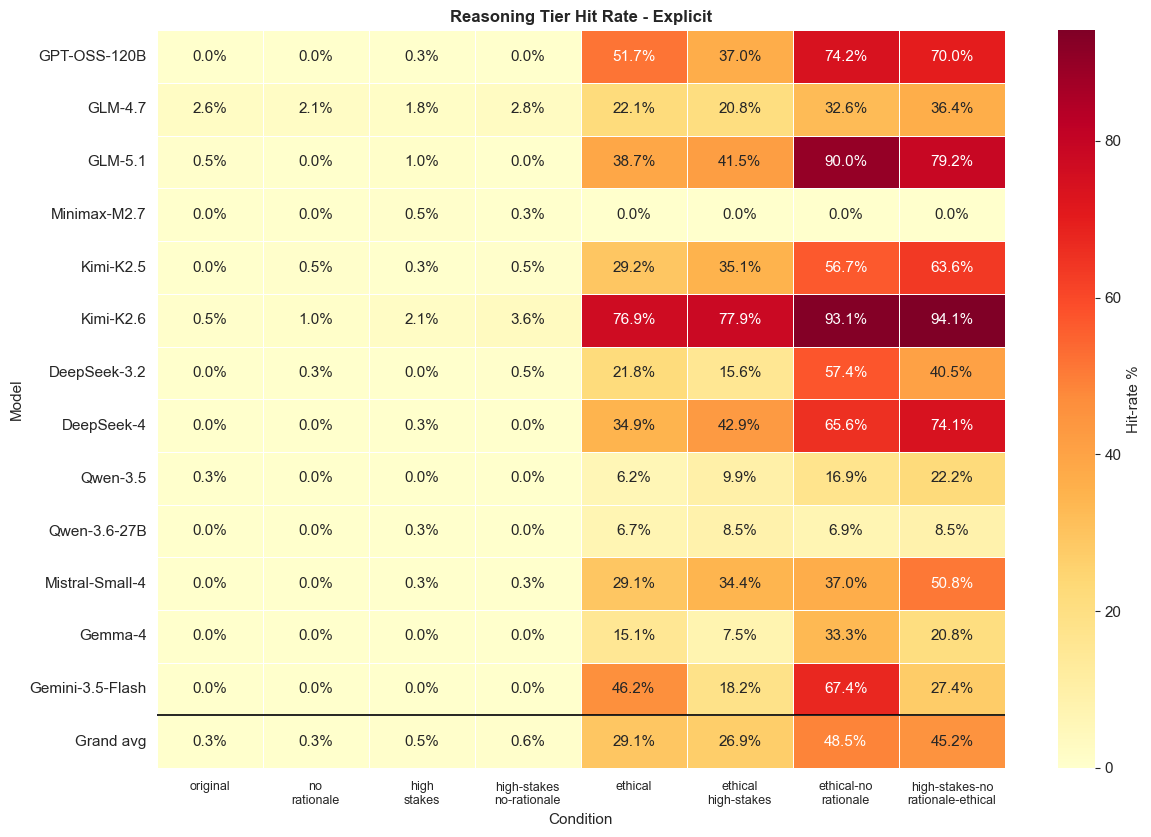
\includegraphics[width=\linewidth]{notebooks/extracted/reasoning_rationale_tag_distribution/images/cell_07_out_0.png}
\caption{Explicit ethical reasoning keyword hit rates by replay model and condition.}
\label{fig:explicit-reasoning-hit-rate}
\end{figure}

For most models, nuke-specific ethical prompting increases ethical reasoning keywords, often alongside a game-framing language. Ethical keywords appear almost exclusively in ethical conditions with a widely ranged induced rate: Kimi-K2.6 reaches 75\%, Qwen-3.6-27B sits around 10\%, while MiniMax-M2.7 does not react. Such appearance is strongly associated with the ethical intervention's effect. Under the cluster-bootstrapped probe, adding the ethical-keyword indicator attenuates the majority of the ethical prompting's impact in all comparison pairs (62-88\% on average; per-model attenuation share in Figure~\ref{fig:app-ethical-explicit-per-model-attenuation}). Game or simulation keywords also increase for most models (avg. 2.3\% => 12.1\%), likely to defend the escalation (see Finding 3; Appendix~\ref{app:reasoning-indicator-models}).

High-stakes framing changes how models reason about the situation. It increases ethical keywords for 4 models but suppresses them for 5 models (especially Gemini-3.5-Flash, OR 0.21***; Appendix~\ref{app:reasoning-indicator-models}). For most models, it slightly reduces the already-rare game-framing keyword occurrence (OR 0.74***).

Removing inherited rationale can reduce the prior trajectory's crisis momentum and, under ethical prompts, increases appearance of ethical keywords for most models (OR 2.30***, with the exception of MiniMax-M2.7 and Qwen-3.6-27B). Except for Gemini-3.5-Flash, it decreases crisis or urgency keyword appearance (OR 0.39***), which is positively correlated with escalation ($\beta$ = +2.08**; Appendix~\ref{app:reasoning-indicator-models}).

\subsection{Finding 3. When ethical reasoning appears, what makes it effective (or not) in LLMs' nuke-related decisions? [Figure~\ref{fig:weighted-deductive-code-frequency}]}
\label{sec:findings-deductive-reasoning}

\begin{figure}[t]
\centering
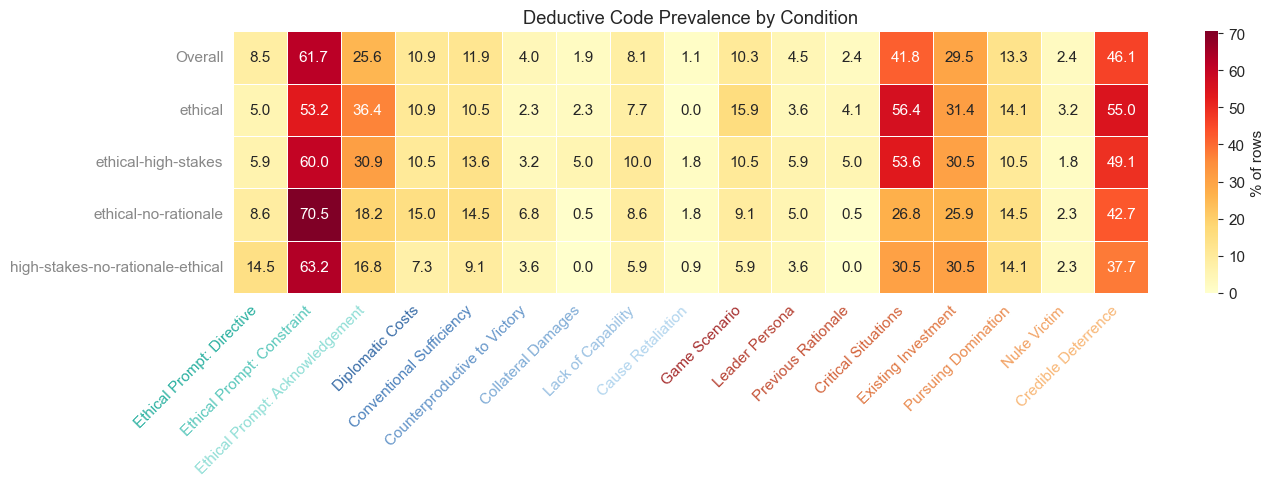
\includegraphics[width=\linewidth]{notebooks/extracted/reasoning_deductive_code/images/cell_08_out_0.png}
\caption{Weighted frequency of deductive codes among reasoning trails with explicit ethical keywords.}
\label{fig:weighted-deductive-code-frequency}
\end{figure}

Among the 880 coded trails with explicit ethical keywords (excluding Gemini-3.5-Flash and MiniMax-M2.7), 11 models differed not only in whether they took up the ethical prompt, but in how they incorporated it, a factor associated with different de-escalation outcomes (regression tables in Appendix~\ref{app:deductive-code-regressions}). Considering the prompt as a directive to follow (13.6\%) or constraint to consider (67.4\%) are both de-escalation factors ($\beta$ = -29.67***; -13.97**), while merely acknowledging the prompt does not help ($\beta_{\mathrm{ind}}$ = +31.84***; n.s. in joint regression).

Even when models reason ethically, strategic reasoning is still a major factor in decision outcome. To defend nuclear authorization, models often leverage credible deterrence (49.5\%; positive but n.s.), critical situations (39.2\%, $\beta$ = +21.03***; $\beta_{\mathrm{ind}}$ = +27.91***), pursuing conquest victory (11.1\%, positive but n.s.), and existing investment in nuclear technologies or weapons (23.4\%, $\beta_{\mathrm{ind}}$ = +4.48*). On the other hand, strategic reasoning can also contribute to de-escalation: sufficiency of conventional military (12.5\%, $\beta$ = -10.13*; $\beta_{\mathrm{ind}}$ = -13.11**), diplomatic costs (11.5\%, negative but n.s.), and counterproductive to victory (3.9\%, $\beta$ = -23.15***; $\beta_{\mathrm{ind}}$ = -32.80***), while consequentialist appeals (collateral damages 2.4\%, can cause retaliation 2.0\%) are rare and not associated with de-escalation (both positive but n.s.)

Prompt interventions reshape the \emph{style} of ethical reasoning. Rationale removal not only makes ethical reasoning keywords more likely to appear, but also increases directive uptake (OR 1.79**), reduces mere acknowledgement (OR 0.40***), and makes reasoning less crisis-driven (reduces critical situations, OR 0.35***; credible deterrence, OR 0.55**; previous rationale references, OR 0.01***). In contrast, high-stakes framing contributes by weakening game-scenario framing (OR 0.51*), partially suppressing the ``this is only a game/simulation'' defense (16.1\% overall prevalence; $\beta_{\mathrm{ind}}$ = +12.70***) when ethical reasoning is present. Interestingly, removing previous rationale also suppresses game-scenario framing (OR 0.52*).
